% ============================================================
% Figures 2 and 3. Upload figures/fig2_field_technology.pdf and
% figures/fig3_communities.pdf to Overleaf, then paste each block where it belongs.
% Regenerate with:  python report/make_fig2.py . report/figures
%                   python report/make_fig3.py . report/figures
% ============================================================


% ---------- RESULTS 2: field or technology ----------
\begin{figure*}[t]
\centering
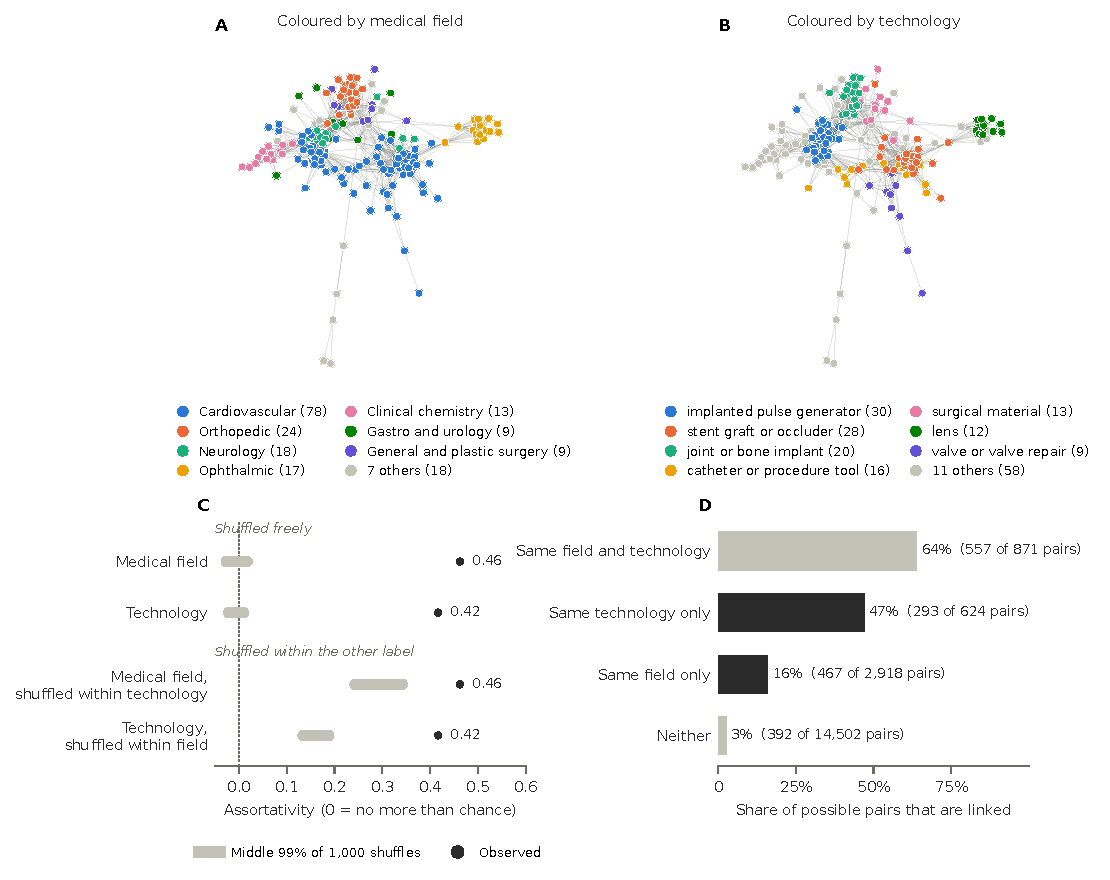
\includegraphics[width=\textwidth]{figures/fig2_field_technology.pdf}
\caption{\textbf{Links follow both medical field and technology, and technology is the stronger link pair by pair.}
(\textit{A}, \textit{B}) The network of Fig.~\ref{fig:network} (largest component, 186 codes), coloured by medical field and by technology. The seven largest categories are in colour; counts in brackets are codes.
(\textit{C}) Assortativity of each label over all 195 linked codes (dots), against 1,000 shuffles of that label (grey bars, middle 99\%). Shuffled freely, both labels are far above chance. Shuffled only among codes that share the other label, which keeps everything the other label explains, each still beats every shuffle ($p \le 0.001$, one-sided), so each label explains links the other does not.
(\textit{D}) Share of possible pairs of codes that are linked, by whether the two codes share a field, a technology, both or neither. Codes that share only a technology are linked three times as often as codes that share only a field (47\% against 16\%). There are, however, about five times fewer such pairs, so field still accounts for more links overall.}
\label{fig:labels}
\end{figure*}


% ---------- RESULTS 3: communities ----------
\begin{figure*}[t]
\centering
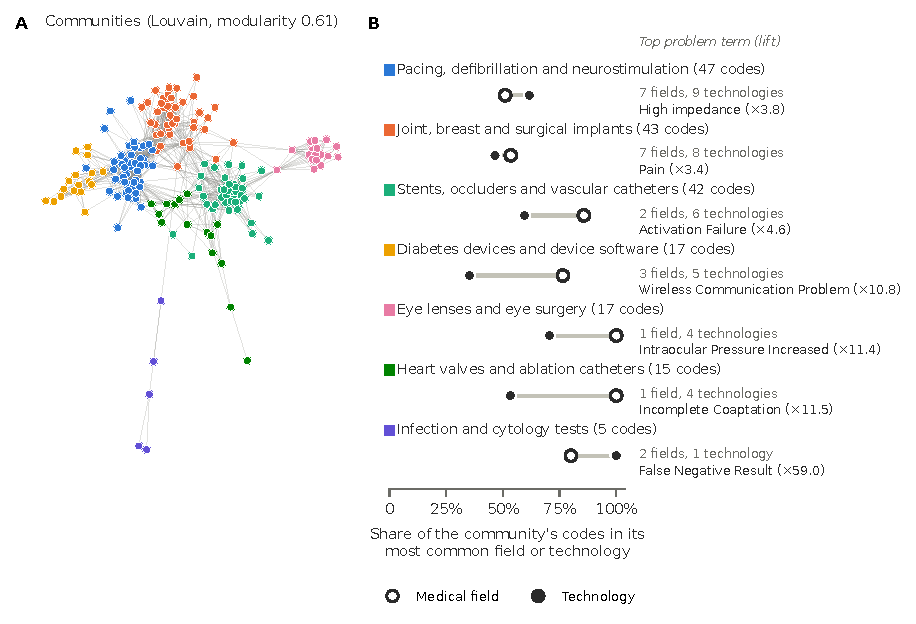
\includegraphics[width=\textwidth]{figures/fig3_communities.pdf}
\caption{\textbf{Communities found without labels stay within one field, except where a technology spans several.}
(\textit{A}) Louvain communities of the network (best of 20 runs, modularity 0.61) on the layout of Fig.~\ref{fig:network}. Three further communities of two to four codes (prostate cancer tests, implanted glucose sensors and mammography) lie outside the largest component and are not shown.
(\textit{B}) For each community of at least five codes: the share of its codes in its most common medical field (open circle) and in its most common technology (filled circle), how many fields and technologies it spans, and the FDA problem term most over-represented in its reports (lift: the term's share among the community's terms divided by its share among all sampled terms, for terms in at least 5\% of the community's reports). Most communities sit mainly in one field. The largest spans seven fields and is held together by technology: 62\% of its codes are implanted pulse generators, while its largest field holds 51\%. Its top problem term, high impedance, describes the electronics rather than the body part.}
\label{fig:communities}
\end{figure*}
